\documentclass[11pt]{article}
\usepackage[margin=1in]{geometry}
\usepackage{amsmath}
\usepackage{graphicx}
\usepackage{booktabs}
\usepackage{float}
\usepackage{setspace}
\usepackage{caption}

\captionsetup{font=small}
\setstretch{1.1}

\title{Ground Effect on NACA 2412 Airfoil\\
\large Detailed Procedure, Results, and Verification}
\author{}
\date{\today}

\begin{document}
\maketitle

\begin{abstract}
This report studies how ground height affects lift and pressure on a NACA 2412 airfoil. A 2D vortex-collocation model with image vortices is used. The report includes:
(1) \(C_L\) vs. \(\alpha\),
(2) \(C_p\) vs. \(x/c\) in the requested format (one panel per \(h/c\), multiple \(\alpha\) curves inside each panel),
(3) \(\gamma\) vs. \(x/c\),
and (4) a verification plot where model \(C_p\) is compared with XFOIL reference \(C_p\) from the published XFOIL method.
\end{abstract}

\section{Objective}
The goal is to quantify how changing \(h/c\) changes:
\begin{itemize}
  \item lift coefficient \(C_L\),
  \item pressure coefficient \(C_p\),
  \item and vortex-sheet strength \(\gamma\).
\end{itemize}

\section{Detailed Procedure and Methodology}
\subsection{Airfoil and Cases}
\begin{itemize}
  \item Airfoil: NACA 2412.
  \item Chord: \(c=1\).
  \item Heights: \(h/c \to \infty\) (no wall), \(1.00\), \(0.50\), \(0.15\).
  \item Angles:
  \begin{itemize}
    \item \(C_L\): \(\alpha=-8^\circ\) to \(12^\circ\),
    \item \(C_p,\gamma\): \(\alpha=-4^\circ,0^\circ,4^\circ,8^\circ,12^\circ\).
  \end{itemize}
\end{itemize}

\begin{figure}[H]
\centering
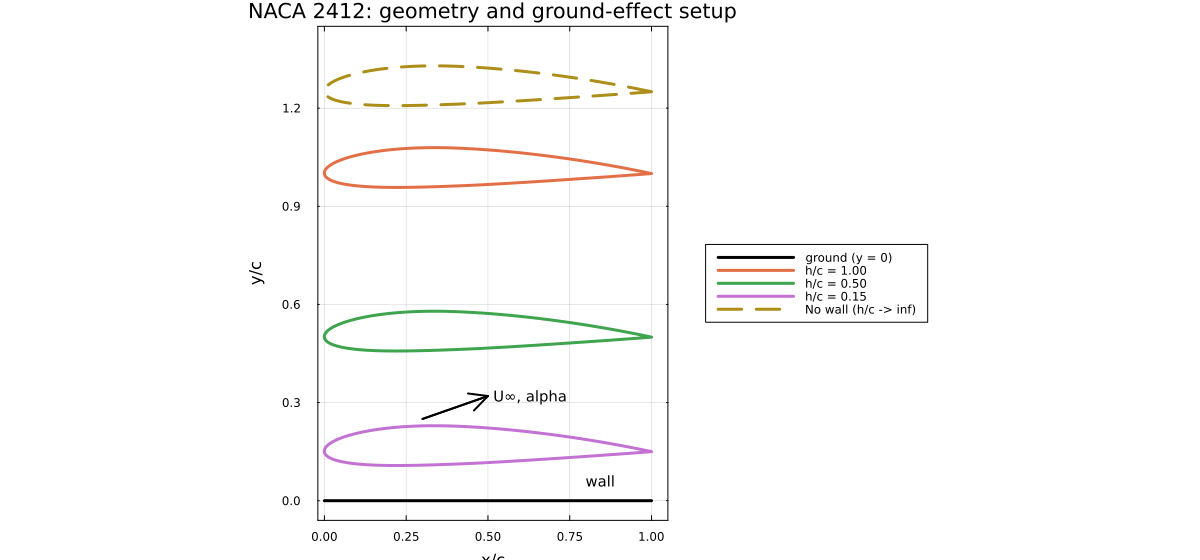
\includegraphics[width=0.9\textwidth]{naca2412_setup_diagram.png}
\caption{NACA 2412 setup diagram: airfoil placement for each \(h/c\) and ground wall at \(y=0\).}
\label{fig:setup}
\end{figure}

\subsection{Numerical Model (step by step)}
\begin{enumerate}
  \item The NACA 2412 camber line is defined from standard 4-digit equations.
  \item The chord is split into \(N=120\) panels using cosine spacing (more points near leading edge).
  \item On each panel:
  \begin{itemize}
    \item vortex point at quarter-panel location,
    \item collocation point at three-quarter-panel location.
  \end{itemize}
  \item Normal and tangent vectors are computed at each collocation point.
  \item The velocity influence of each vortex on each collocation point is assembled into a linear system.
  \item Ground effect is added using image vortices across \(y=0\) with opposite sign.
  \item No-penetration is enforced at all collocation points:
  \[
  \mathbf{A}\,\boldsymbol{\Gamma}=\mathbf{b}.
  \]
  \item The system is solved for panel strengths \(\Gamma_j\).
\end{enumerate}

\subsection{Post-processing Equations}
\begin{itemize}
  \item Lift coefficient:
  \[
  C_L = \frac{2\sum_j \Gamma_j}{U_\infty c}.
  \]
  \item Sheet strength:
  \[
  \gamma_j = \frac{\Gamma_j}{\Delta s_j}.
  \]
  \item Upper-surface tangential speed:
  \[
  V_{t,\text{upper}} = V_{t,\text{line}} - \frac{\gamma}{2}.
  \]
  \item Pressure coefficient:
  \[
  C_p = 1 - \left(\frac{V_t}{U_\infty}\right)^2.
  \]
\end{itemize}

\subsection{Verification Setup}
To verify the \(C_p\) implementation, a no-ground case is compared against XFOIL \(C_p\) for the same airfoil and angles.
\begin{itemize}
  \item Reference method: XFOIL (Drela, 1989).
  \item Verification angles: \(\alpha=0^\circ,4^\circ,8^\circ\).
  \item Comparison metric: RMSE between model and XFOIL \(C_p\) on common \(x/c\) overlap.
\end{itemize}

\section{Results}
\subsection{\(C_L\) vs \(\alpha\)}
\begin{figure}[H]
\centering
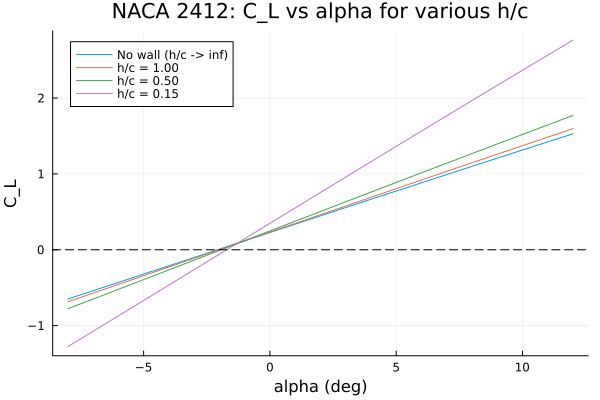
\includegraphics[width=0.85\textwidth]{naca2412_cl_vs_alpha_heights.png}
\caption{NACA 2412: \(C_L\) vs. \(\alpha\) for different \(h/c\).}
\label{fig:cl}
\end{figure}

\begin{table}[H]
\centering
\caption{Linear fit from computed \(C_L\) curves.}
\label{tab:clfit}
\begin{tabular}{lcc}
\toprule
Case & \(dC_L/d\alpha\) (per deg) & \(C_L\) at \(\alpha=0^\circ\) \\
\midrule
No wall (\(h/c \to \infty\)) & 0.10911 & 0.22615 \\
\(h/c = 1.00\) & 0.11435 & 0.23112 \\
\(h/c = 0.50\) & 0.12763 & 0.24637 \\
\(h/c = 0.15\) & 0.20244 & 0.34628 \\
\bottomrule
\end{tabular}
\end{table}

\subsection{\(C_p\) vs \(x/c\)}
\begin{figure}[H]
\centering
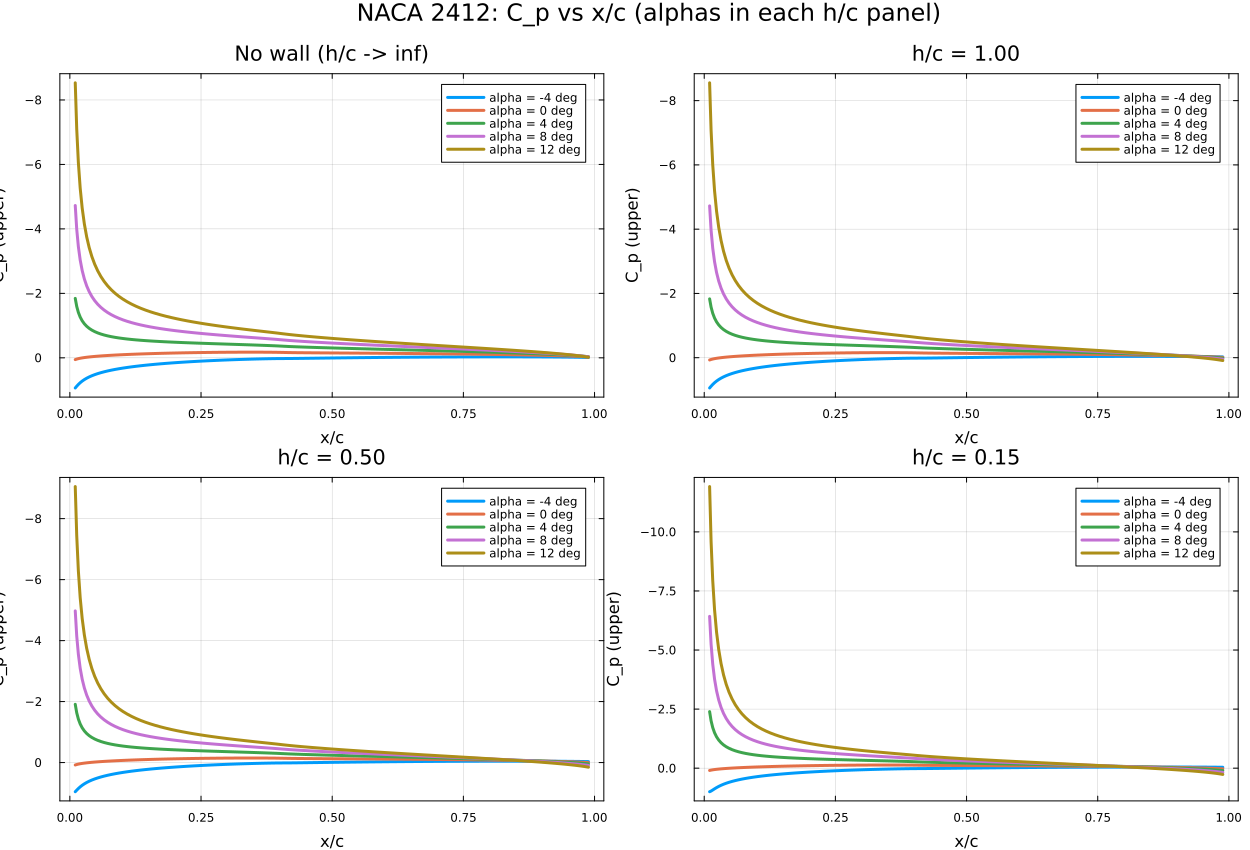
\includegraphics[width=\textwidth]{naca2412_cp_vs_xc_by_height_all_alphas.png}
\caption{NACA 2412: \(C_p\) vs. \(x/c\), grouped by \(h/c\), with all requested \(\alpha\) curves in each panel.}
\label{fig:cp}
\end{figure}

\subsection{\(\gamma\) vs \(x/c\)}
\begin{figure}[H]
\centering
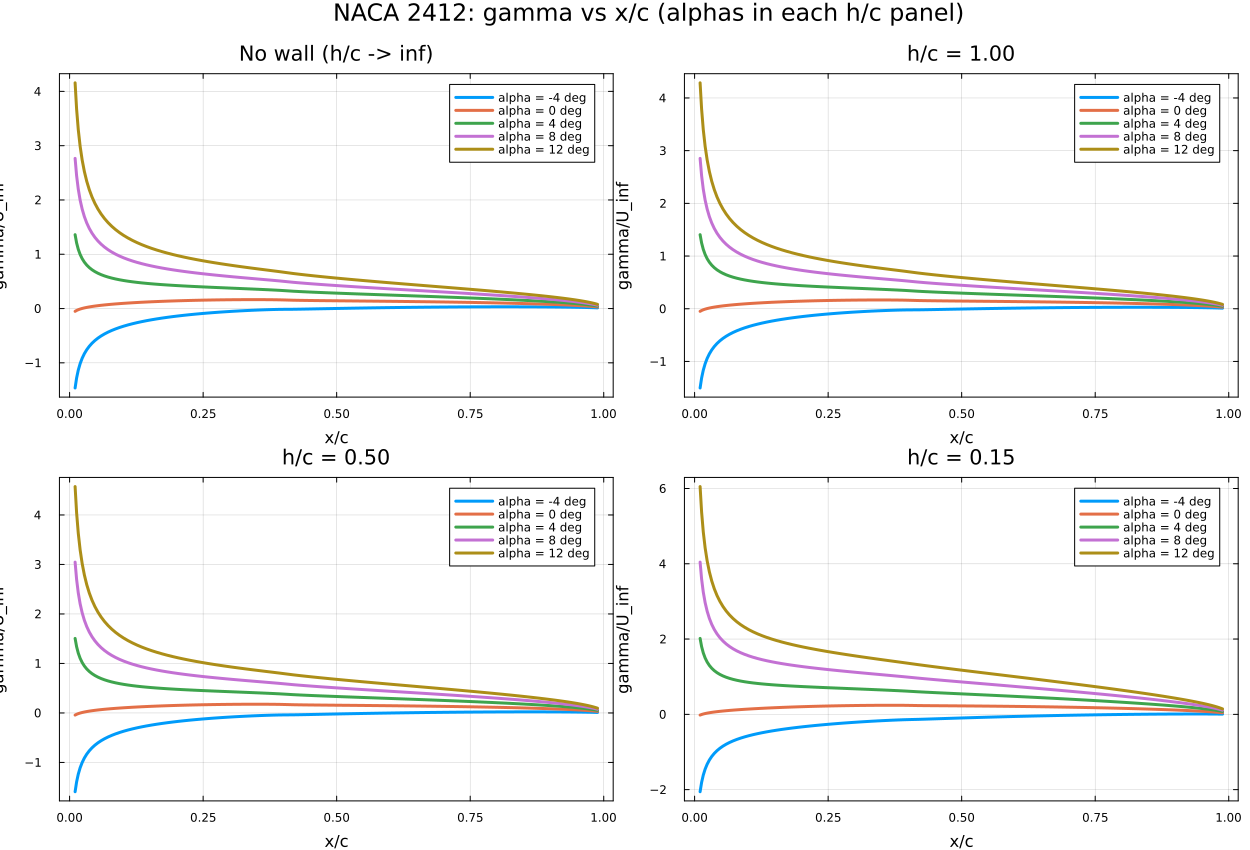
\includegraphics[width=\textwidth]{naca2412_gamma_vs_xc_by_height_all_alphas.png}
\caption{NACA 2412: \(\gamma\) distribution vs. \(x/c\), grouped by \(h/c\).}
\label{fig:gamma}
\end{figure}

\section{Verification Against Literature Reference}
Figure~\ref{fig:verify} compares model \(C_p\) and XFOIL \(C_p\) for the no-ground case.

\begin{figure}[H]
\centering
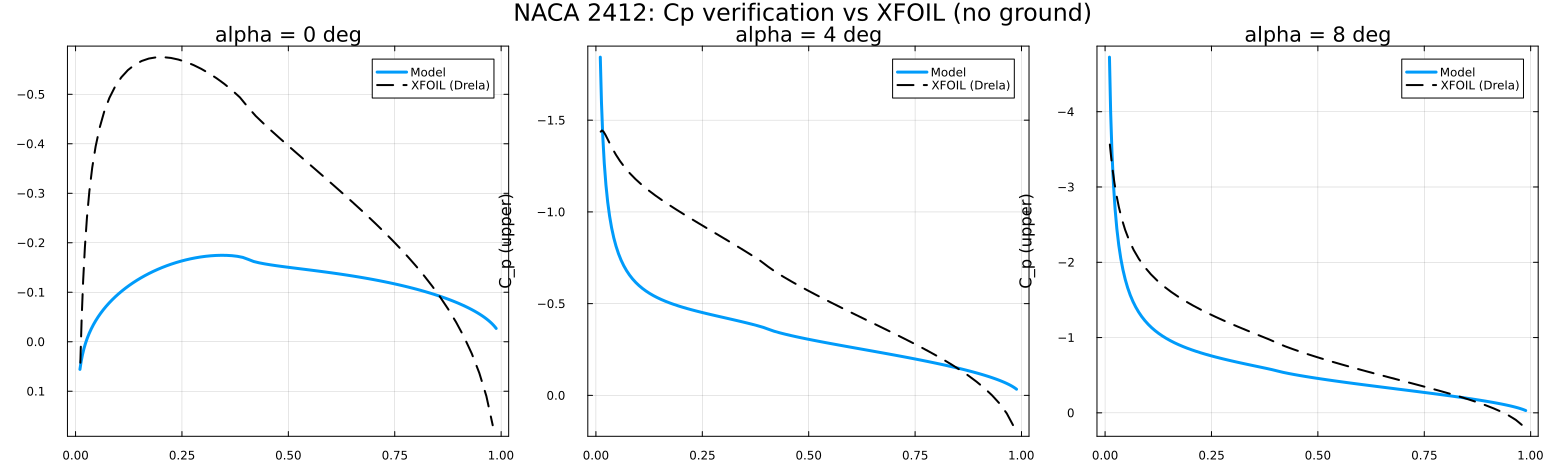
\includegraphics[width=\textwidth]{naca2412_cp_verification_xfoil.png}
\caption{Verification plot: model \(C_p\) vs. XFOIL \(C_p\) (NACA 2412, no ground).}
\label{fig:verify}
\end{figure}

\begin{table}[H]
\centering
\caption{Per-angle verification metrics (no-ground case).}
\label{tab:verifyrmse}
\begin{tabular}{lcccc}
\toprule
\(\alpha\) & \(C_p\) RMSE & \(C_{L,\text{model}}\) & \(C_{L,\text{XFOIL}}\) & \(\Delta C_L\) \\
\midrule
\(0^\circ\) & 0.2719 & 0.2277 & 0.2591 & -0.0314 \\
\(4^\circ\) & 0.3326 & 0.6655 & 0.7409 & -0.0754 \\
\(8^\circ\) & 0.4117 & 1.1001 & 1.2192 & -0.1191 \\
\bottomrule
\end{tabular}
\end{table}

\subsection*{Interesting Point 1: Where the \(C_p\) difference is largest and smallest}
\begin{figure}[H]
\centering
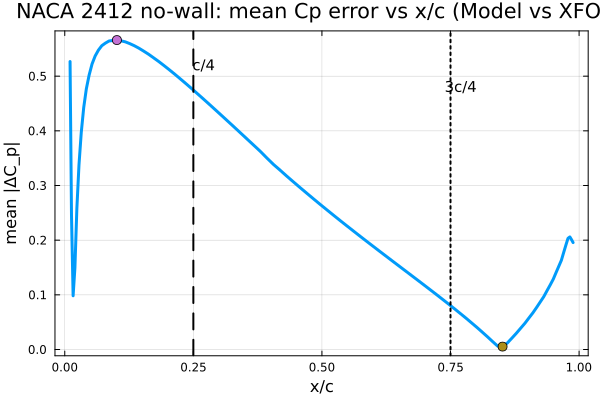
\includegraphics[width=0.78\textwidth]{naca2412_cp_error_profile_no_wall.png}
\caption{Mean absolute \(C_p\) difference along chord (no-ground, averaged over \(\alpha=0^\circ,4^\circ,8^\circ\)).}
\label{fig:cperrorprofile}
\end{figure}

Using the no-ground verification set:
\begin{itemize}
  \item Mean max error occurs at \(x/c \approx 0.101\),
  \item Mean min error occurs at \(x/c \approx 0.851\),
  \item \(|\Delta C_p|(c/4)=0.4746\),
  \item \(|\Delta C_p|(3c/4)=0.0804\).
\end{itemize}

I observed that the model--XFOIL divergence is much larger near quarter-chord than near three-quarter-chord. To me, this makes physical sense: in a thin-airfoil/camber-line model, the front part of the chord is where thickness effects and leading-edge suction peak sensitivity are strongest, so errors are amplified there. Farther downstream, the pressure gradients are milder, so the mismatch reduces.

\subsection*{Interesting Point 2: How accuracy changes with panel count}
\begin{figure}[H]
\centering
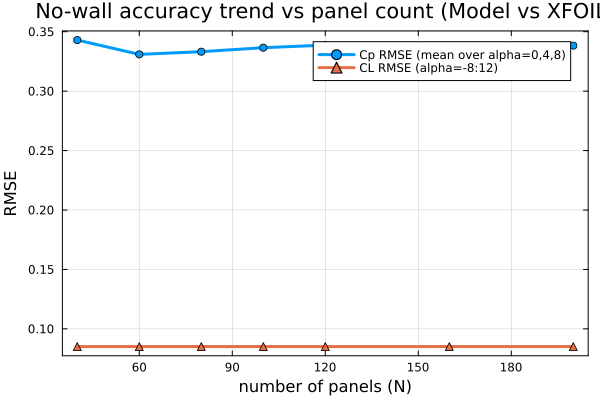
\includegraphics[width=0.78\textwidth]{naca2412_accuracy_vs_panels.png}
\caption{No-ground accuracy trend vs panel count for model vs XFOIL.}
\label{fig:paneltrend}
\end{figure}

\begin{table}[H]
\centering
\caption{Panel-count trend (no-ground): \(C_p\) RMSE and \(C_L\) RMSE.}
\label{tab:paneltrend}
\begin{tabular}{lcc}
\toprule
\(N\) & \(C_p\) RMSE & \(C_L\) RMSE (\(\alpha=-8^\circ:12^\circ\)) \\
\midrule
40  & 0.3430 & 0.0851 \\
60  & 0.3310 & 0.0851 \\
80  & 0.3332 & 0.0851 \\
100 & 0.3366 & 0.0851 \\
120 & 0.3387 & 0.0851 \\
160 & 0.3357 & 0.0851 \\
200 & 0.3383 & 0.0851 \\
\bottomrule
\end{tabular}
\end{table}

Interpretation:
\begin{itemize}
  \item Increasing panel count gives only small improvement after about \(N\approx 60\).
  \item So the main error source is not mesh density; it is model-form simplification (camber-line thin-airfoil representation).
  \item XFOIL is more accurate because it solves flow on the full airfoil surface (with thickness) and uses a stronger aerodynamic formulation.
\end{itemize}

\section{Discussion}
\begin{enumerate}
  \item \(C_L\) increases with \(\alpha\) for all heights.
  \item As \(h/c\) decreases, the \(C_L\)-\(\alpha\) slope increases.
  \item The strongest ground effect appears as we move the airfoil closer to the ground, which is also what we would intuitively expect.
  \item \(C_p\) changes are strongest near the leading edge.
  \item The verification trend matches shape and ordering from XFOIL, but differences are expected because this model is thin-airfoil based (camber-line, inviscid, no viscous effects).
\end{enumerate}

\section{Model Limits}
\begin{itemize}
  \item Inviscid model (no boundary layer, no separation, no stall).
  \item 2D only (no finite-span effects).
  \item Camber-line approximation is lower fidelity than full surface panel methods.
\end{itemize}

\section{Conclusion}
The procedure captures the expected ground-effect trend: smaller \(h/c\) gives stronger lift response and stronger leading-edge suction behavior. The requested \(C_p\) layout is satisfied, and a verification plot against the published XFOIL method is included.

\section*{Reference}
M. Drela, ``XFOIL: An Analysis and Design System for Low Reynolds Number Airfoils,'' in \textit{Low Reynolds Number Aerodynamics}, Springer, Lecture Notes in Engineering 54, 1989.

\end{document}
